\subsection{M.PC.11 - Rischi inattesi}
\begin{figure}[H]
    \centering
    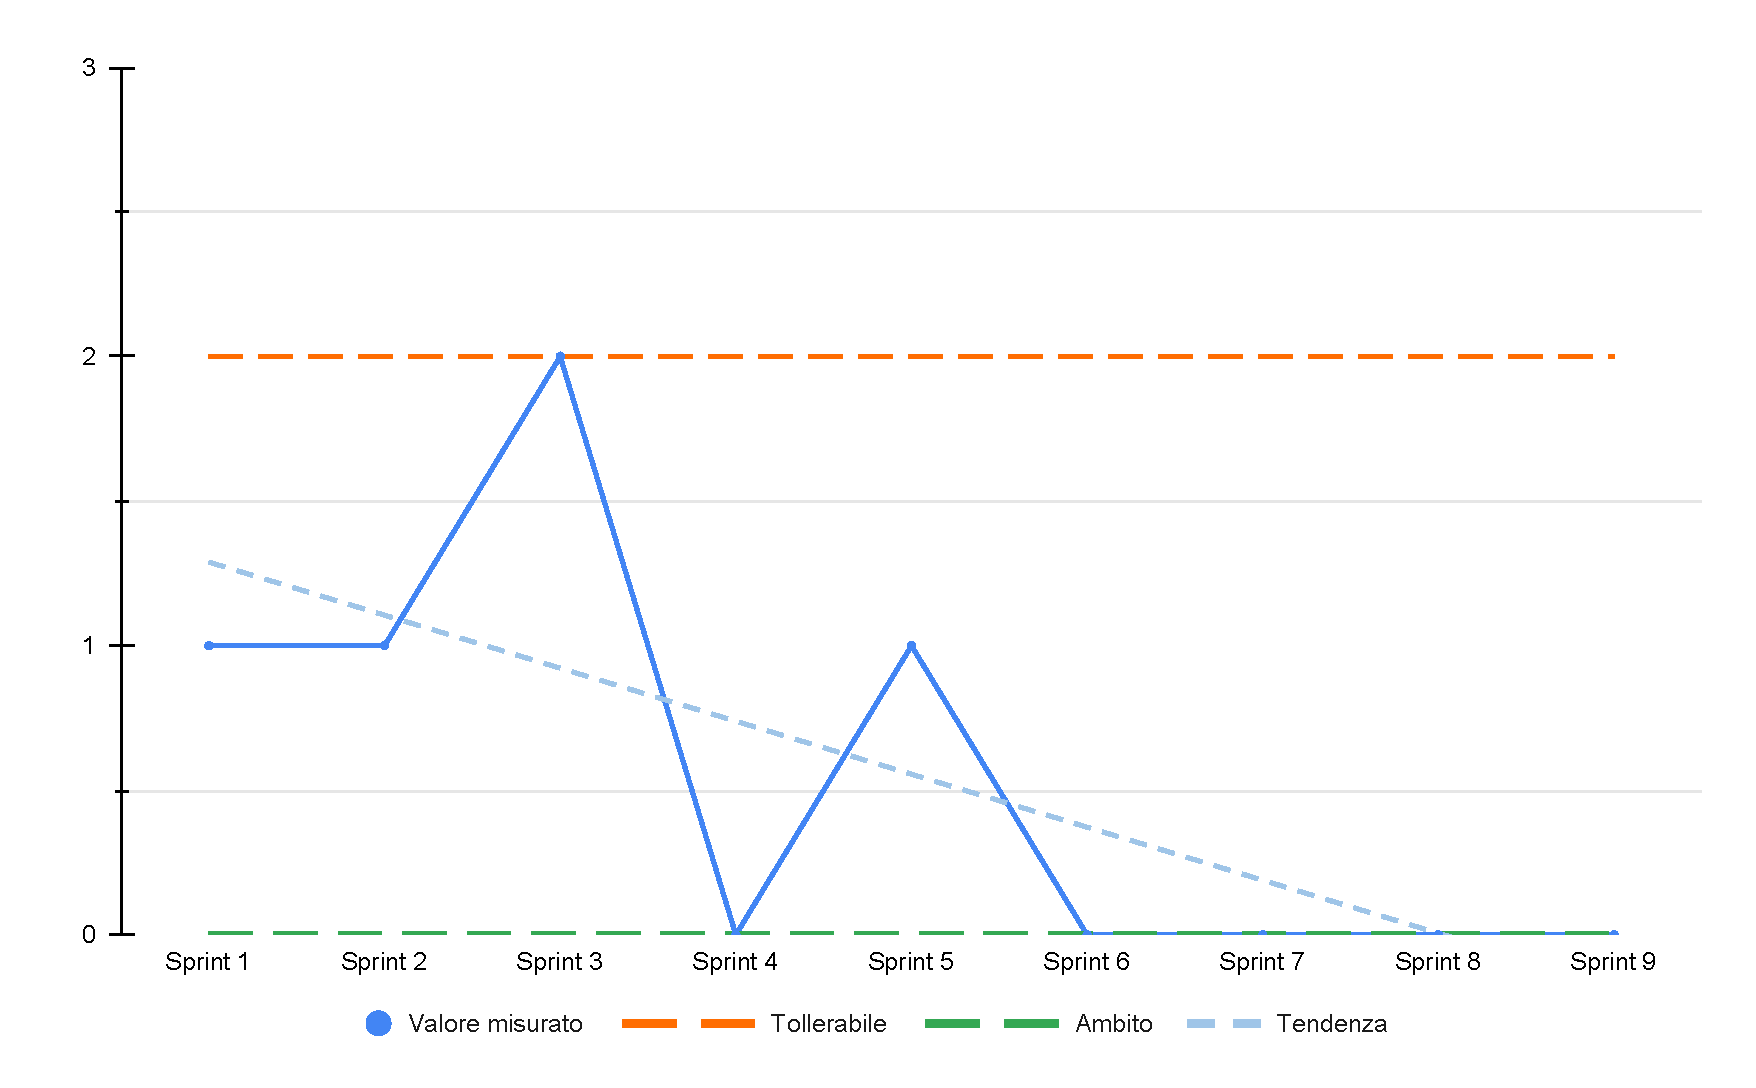
\includegraphics[width=\textwidth]{assets/rischi_inattesi.pdf}
    \caption{M.PC.11 - Rischi inattesi}
\end{figure}

\par Fino al quarto \glossario{sprint}, il team ha dovuto affrontare almeno un rischio inatteso. Tuttavia, il numero di rischi non previsti è sempre stato inferiore rispetto alla soglia tollerabile. Dallo \glossario{sprint} 5, invece, tutti i rischi che si sono verificati erano già stati analizzati e documentati nel \textit{Piano di Progetto}. Questo ha permesso al team una migliore gestione del progetto. Di conseguenza, a partire dal settimo \glossario{sprint}, il gruppo ha deciso di abbassare il valore tollerabile a 1. L'obiettivo per le iterazioni successive, infatti, è mantenere il numero di rischi inattesi quanto più stabile e prossimo al valore ambito.